\documentclass[11pt]{article}
\usepackage{amsmath}
\usepackage{graphicx}
\usepackage{geometry}
\usepackage[hidelinks]{hyperref}
\usepackage{titlesec}
\usepackage{amssymb}
\usepackage{algorithm}
\usepackage{algpseudocode}
\usepackage{multirow}
\geometry{margin=1in}
\titleformat{\section}{\normalfont\Large\bfseries}{\thesection}{1em}{}
\titleformat{\subsection}{\normalfont\large\bfseries}{\thesubsection}{1em}{}

\title{Optimization Techniques: Exercise 2}
\author{Maria Charisi 10727}
\date{November 2025\\ 
\href{https://github.com/mariaxarisi/Optimization-Techniques}{\texttt{Github Repo}}}

\begin{document}

\maketitle

\begin{abstract}
This report constitutes the second part of the assignment for the \textit{Optimization Techniques} course at the \textit{Aristotle University of Thessaloniki}. 
In this work, we implement and analyze the performance of some optimization methods that make use of derivative information in order to locate the global minimum of multivariable functions. 
Through numerical experiments, we compare the behavior of these algorithms under different initialization points and step–size selection rules, highlighting their convergence characteristics and effectiveness.
\end{abstract}


\tableofcontents
\newpage

\section{Introduction}

In this assignment we focus on the study and implementation of the following optimization methods:
\begin{itemize}
    \item Steepest Descent Method,
    \item Newton's Method,
    \item Levenberg--Marquardt Method.
\end{itemize}

All of these algorithms are based on the general idea of \textit{iterative descent}.  
In iterative descent methods, we begin from an initial point $x_0 \in \mathbb{R}^n$ and generate a sequence of points
\(
x_0,\, x_1,\, x_2,\, \ldots
\)
such that the objective function decreases monotonically, i.e.
\[
f(x_{k+1}) < f(x_k), \qquad k = 0,1,2,\ldots,
\]
so that after a number of iterations the sequence approaches a (local) minimum of the function.

Each new vector is computed according to the update rule
\[
x_{k+1} = x_k + \gamma_k d_k,
\]
where $d_k$ is the \textit{descent direction}, which satisfies the condition
\(
\nabla f(x_k)^\top d_k < 0,
\)
and $\gamma_k>0$ is the \textit{step size} (or learning rate), which ensures that
\(
f(x_k + \gamma_k d_k) < f(x_k).
\)

The choice of the step size $\gamma_k$ is crucial for the behavior of the algorithm.  
A step size that is too small leads to very slow progress and therefore slow convergence.  
On the other hand, a step size that is too large may cause the algorithm to diverge or overshoot the region where the function decreases and never converge.

For each of the three main optimization methods, we examine three different strategies for determining the step size:
\begin{itemize}
    \item \textbf{Fixed Step:} a constant value of $\gamma_k = \gamma$ is used at every iteration.
    
    \item \textbf{Optimal Step:} at every iteration, the step size $\gamma_k$ is chosen to minimize the function along the descent direction:
    \[
    \gamma_k = \arg \min_{\gamma > 0} f(x_k + \gamma d_k).
    \]

    \item \textbf{Armijo Rule:} the step size is chosen according to
    \(
    \gamma_k = s \beta^{\mu_k},
    \)
    where $\mu_k$ is the smallest non-negative integer satisfying the Armijo condition
    \[
    f(x_k + \gamma_k d_k) 
    \le f(x_k) + \alpha \gamma_k \nabla f(x_k)^\top d_k .
    \]
    Here $s$ is an initial step size, the parameter $\alpha$ is typically chosen in the interval $\alpha \in [10^{-5}, 10^{-1}]$, and $\beta$ is chosen in the range $\beta \in [\tfrac{1}{10},\, \tfrac{1}{2}]$.
\end{itemize}

\subsection{Objective Function}

Given the three initial starting points $[0,0]$, $[-1,-1]$, and $[1,1]$, the goal is to minimize the function
\[
f(x,y) = x^3 e^{-x^2 - y^4}.
\]

The function $f$ is twice continuously differentiable, which is necessary for applying the optimization algorithms examined in this report.
Figures~\ref{fig:3dplot} and \ref{fig:contourplot} show its surface in 3-dimensional space and its contour map in the plane.

For positive values of $x$, the function forms a smooth hill, whereas for negative values of $x$ a deep valley appears.  
This valley contains a single local minimum, numerically approximated at
\[
(x^*,\, y^*) \approx (-1.224570,\; -0.0887658),
\qquad
f(x^*,y^*) = -0.4098908.
\]

\begin{figure}[h!]
    \centering
    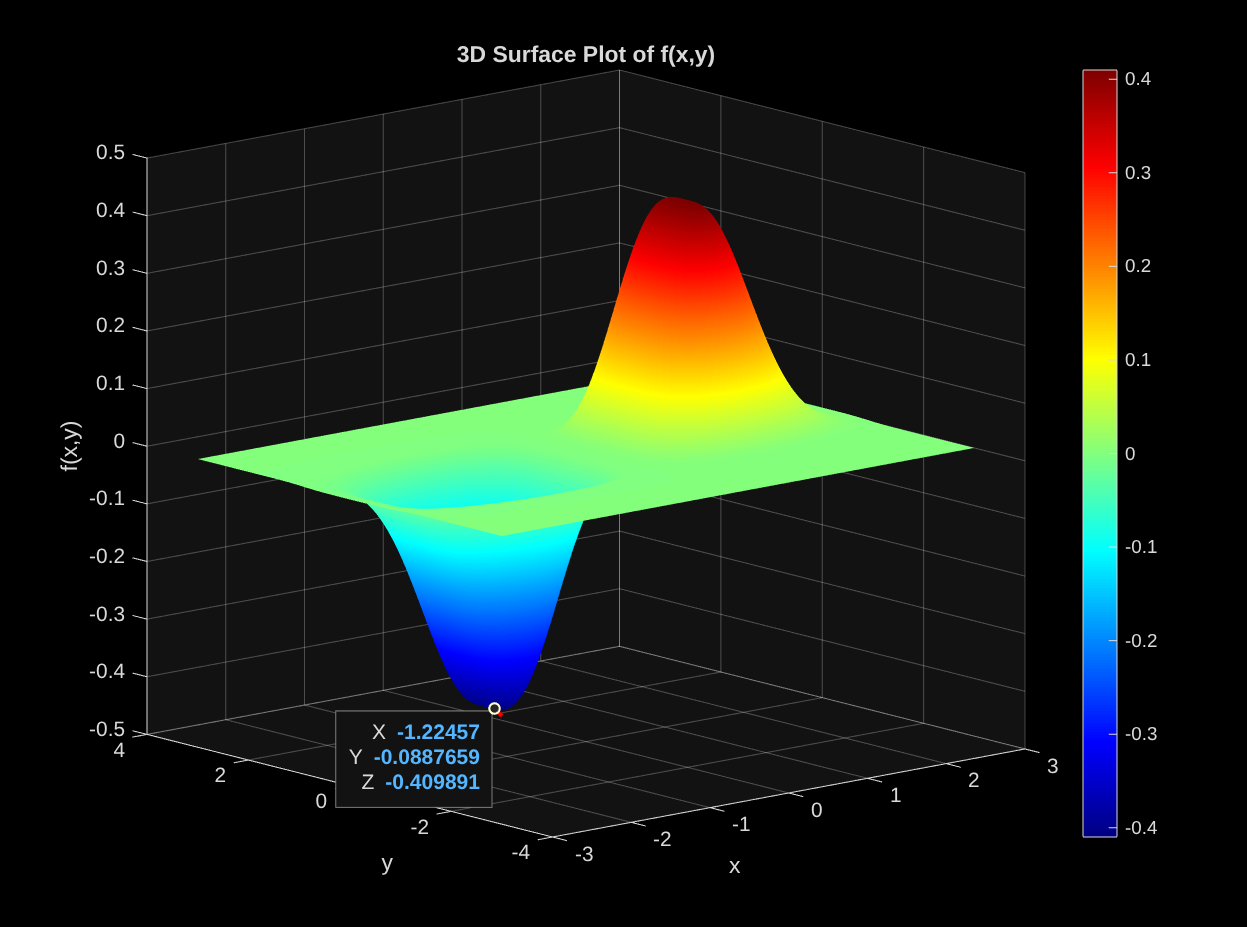
\includegraphics[width=0.75\textwidth]{assets/3D_plot.png}
    \caption{3D surface plot of $f(x,y)$.  
    The deep valley on the left side contains the global minimum.}
    \label{fig:3dplot}
\end{figure}

\begin{figure}[h!]
    \centering
    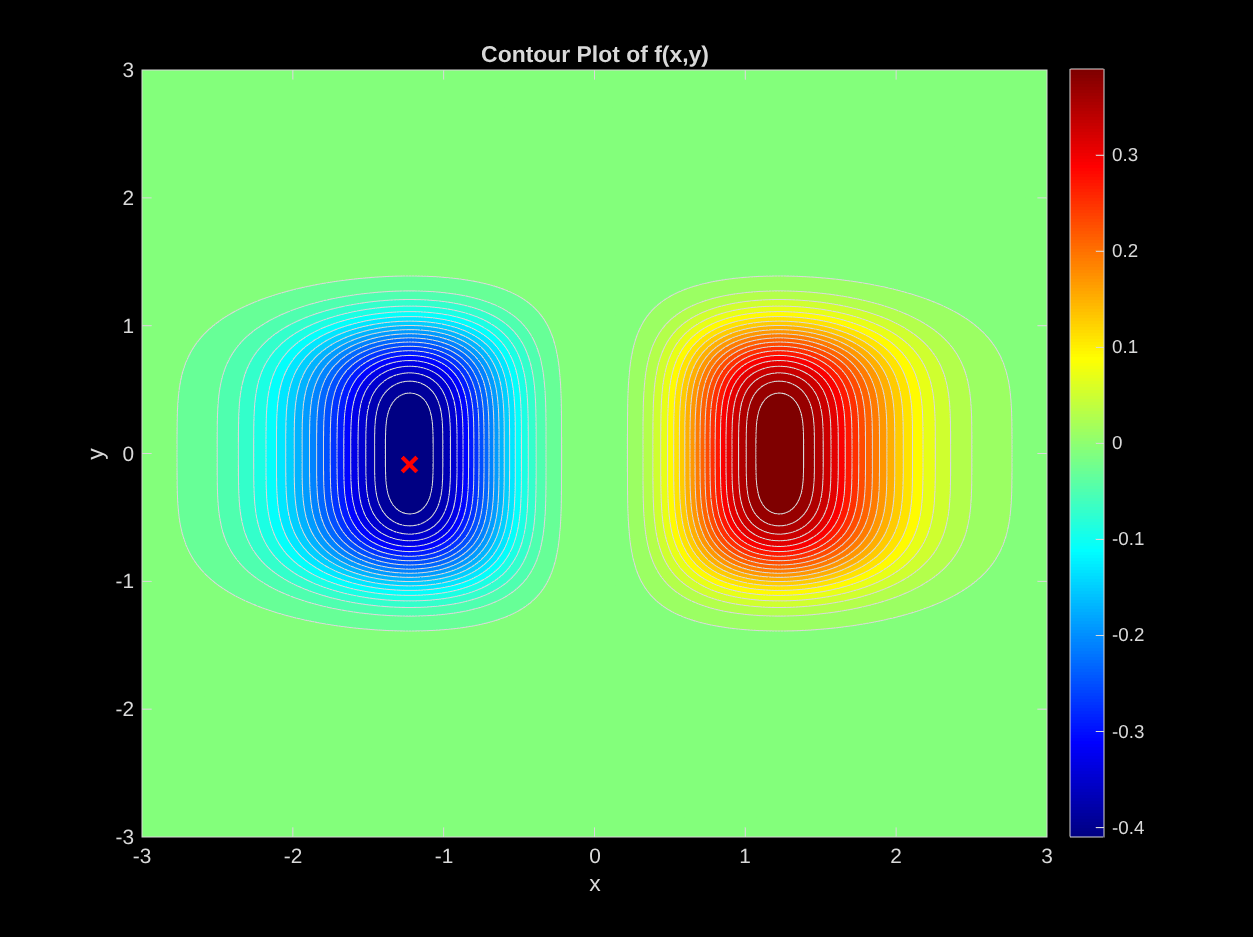
\includegraphics[width=0.75\textwidth]{assets/contour_plot.png}
    \caption{Contour plot of $f(x,y)$.}
    \label{fig:contourplot}
\end{figure}

\newpage
\section{Steepest Descent Method}

\subsection{Method Description}

The Steepest Descent method is one of the simplest iterative optimization algorithms.
At each iteration, the descent direction is chosen as the negative gradient of the
objective function, that is,
\[
d_k = -\nabla f(x_k).
\]

Therefore, the update rule becomes
\[
x_{k+1} = x_k - \gamma_k \nabla f(x_k),
\]
where $\gamma_k > 0$ is the step size, computed using one of the
strategies described in the previous section.

A well–known drawback of the Steepest Descent method is its tendency to produce 
a ``zig–zag'' path toward the minimum.  
This happens because consecutive search directions are orthogonal:
\[
(x_{k+1} - x_k) \perp (x_{k+2} - x_{k+1}),
\]
which often results in slow convergence, especially in narrow or elongated valleys.

\begin{algorithm}[H]
\caption{Steepest Descent Method}
\begin{algorithmic}[1]
\Require Function $f$, gradient $\nabla f$, initial point $x_0$, tolerance $\epsilon > 0$
\Ensure Approximate minimizer $x^*$
\State Set $x_k \gets x_0$, $k \gets 0$
\While{$\|\nabla f(x_k)\| > \epsilon$}
    \State Compute gradient $\nabla f(x_k)$
    \State $d_k \gets -\nabla f(x_k)$ \Comment{Descent direction}
    \State Compute step size $\gamma_k$ (fixed, optimal, or Armijo)
    \State $x_{k+1} \gets x_k + \gamma_k d_k$
    \State $k \gets k + 1$
\EndWhile
\State \Return $x^* \gets x_k$
\end{algorithmic}
\end{algorithm}

\subsection{Results}

In Table~\ref{table:steepest-descent} we present the numerical results obtained by 
applying the Steepest Descent method using the three step–size strategies: fixed step,
optimal step, and Armijo rule. 
For all experiments we used a termination threshold 
$\epsilon = 0.01$; for the fixed step strategy we set $\gamma = 0.1$, and for the Armijo
rule we used the parameters $\alpha = 0.01$ and $\beta = 0.3$.

\begin{table}[h!]
\centering
\begin{tabular}{c|c|c|c|c}
\textbf{Initial Point} & \textbf{Step Type} & \textbf{Minimum Point $x^*$} & \textbf{Minimum Value $f(x^*)$} & \textbf{Iterations} \\
\hline
$(0,0)$ & Fixed   & $(0,\;0)$      & $0$      & $1$ \\
$(0,0)$ & Optimal & $(0,\;0)$      & $0$      & $1$ \\
$(0,0)$ & Armijo  & $(0,\;0)$      & $0$      & $1$ \\
\hline
$(-1,-1)$ & Fixed   & $(-1.224745,\;-0.181086)$   & $-0.409476$     & $92$ \\
$(-1,-1)$ & Optimal & $(-1.224570,\;-0.088766)$   & $-0.409891$     & $2$ \\
$(-1,-1)$ & Armijo  & $(-1.224745,\;-0.181086)$   & $-0.409476$     & $92$ \\
\hline
$(1,1)$ & Fixed   & $(0.905152,\;1.583190)$      & $0.000611$      & $89$ \\
$(1,1)$ & Optimal & $(0.729335,\;2.082661)$      & $0$      & $2$ \\
$(1,1)$ & Armijo  & $(0.905152,\;1.583190)$      & $0.000611$      & $89$ \\
\end{tabular}
\caption{Results of the Steepest Descent method for different step-size strategies.}
\label{table:steepest-descent}
\end{table}

Figure~\ref{fig:steepest-descent} illustrates the convergence behavior of the 
objective function for all initial points and all step-size selection rules.
The horizontal axis represents the iteration number, while the vertical axis shows the 
value of the objective function.  
A red dashed line marks the true minimum value $f_{\min} = -0.4098908$, allowing visual 
comparison between the computed and exact minima.

\begin{figure}[h!]
    \centering
    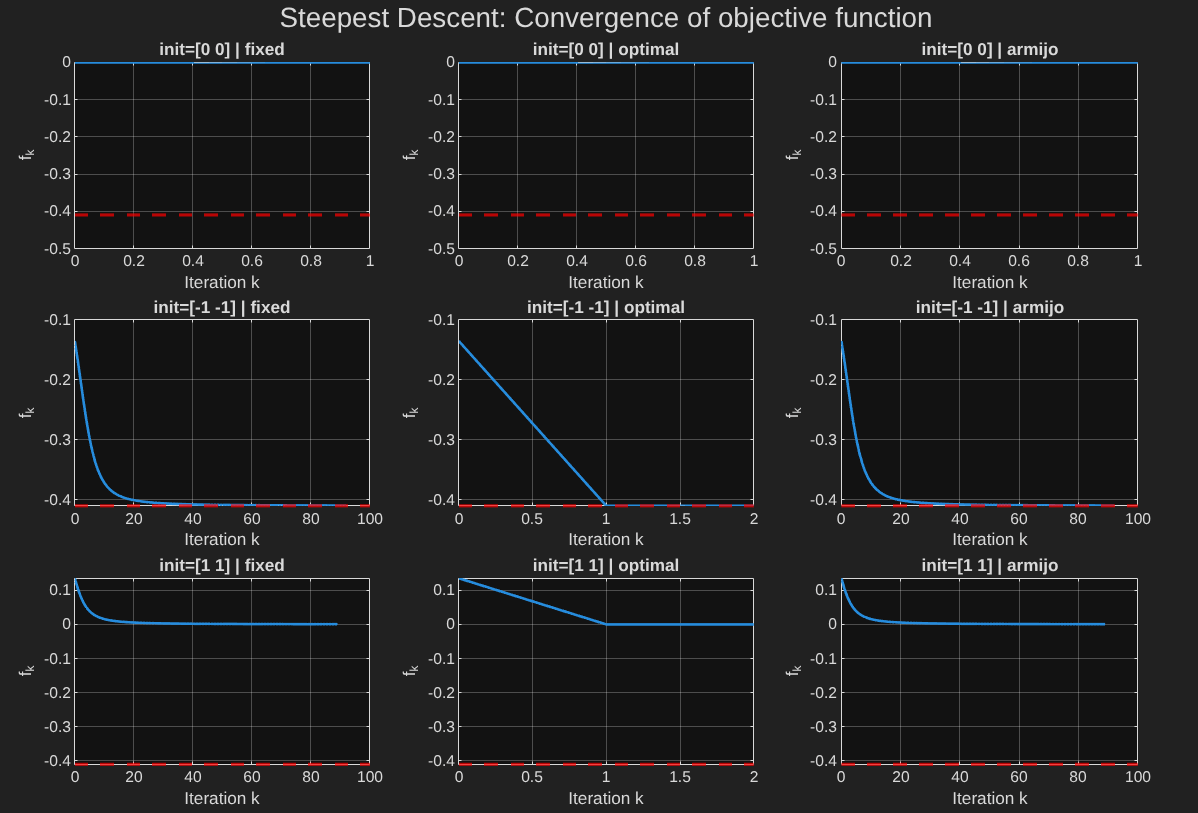
\includegraphics[width=0.95\textwidth]{assets/steepest_descent.png}
    \caption{Convergence of the objective function $f(x,y)$ for different step-size strategies.}
    \label{fig:steepest-descent}
\end{figure}

\newpage
\subsection{Conclusions}

From the experiments with the Steepest Descent method, several important observations can be made regarding the influence of the initial point and the choice of step-size strategy.

\paragraph{Influence of Initial Point} The selection of the initial point significantly affects the outcome of the algorithm:
\begin{itemize}
    \item \textbf{Initial point $(0,0)$:} This point lies in a region where the gradient of $f$ is zero. Consequently, the termination condition $\|\nabla f(x_k)\| < \epsilon$ is satisfied immediately, and the algorithm exits without approaching the absolute minimum.
    
    \item \textbf{Initial point $(-1,-1)$:} For this starting point, all step-size strategies converge close to the absolute minimum
    \[
    (x^*,\, y^*) \approx (-1.224570,\; -0.0887658), \qquad f(x^*,y^*) = -0.4098908.
    \]
    The method successfully finds the global minimum, although the number of iterations depends strongly on the step-size selection. In particular, both the fixed step and the Armijo rule require 92 iterations, whereas the optimal step converges in just 2 iterations.
    
    \item \textbf{Initial point $(1,1)$:} Starting from this point does not lead to the absolute minimum. The fixed step and Armijo rule converge to $(0.905152,\;1.583190)$ with $f \approx 0.000611$, while the optimal step converges to $(0.729335,\;2.082661)$ with $f \approx 0$. Both points are located in flat regions near the hill of the function, far from the global minimum. This behavior occurs because the method initially moves away from the minimum and becomes trapped in regions where the gradient is nearly zero. Once again, the Armijo and fixed step strategies require 89 iterations, while the optimal step converges in only 2 iterations.
\end{itemize}

\paragraph{General Observations}
\begin{itemize}
    \item The initial point selection strongly influences the convergence outcome.
    \item The optimal step-size strategy converges extremely quickly compared to the fixed step and Armijo rule, even though it may converge to a non-optimal point.
    \item The choice of the termination threshold $\epsilon$ affects the number of iterations: a smaller $\epsilon$ forces the method to iterate longer, even if the function value is already close to the minimum.
    \item Overall, the Steepest Descent method is effective primarily when the initial point is near the region of the absolute minimum. Otherwise, it may converge to regions far from the global minimum.
\end{itemize}

\section{Newton's Method}

\subsection{Method Description}

Newton's Method is an iterative optimization algorithm that uses second-order derivative information of the objective function to determine the descent direction.  
At each iteration, the descent direction is computed as

\[
d_k = -[\nabla^2 f(x_k)]^{-1} \nabla f(x_k),
\]

where $\nabla f(x_k)$ is the gradient vector and $\nabla^2 f(x_k)$ is the Hessian matrix evaluated at $x_k$.  

Accordingly, the update rule becomes

\[
x_{k+1} = x_k - \gamma_k [\nabla^2 f(x_k)]^{-1} \nabla f(x_k),
\]

where $\gamma_k > 0$ is the step size, which can be determined using a fixed value, an optimal line search, or the Armijo rule.

The primary drawback of Newton's Method arises when the Hessian matrix is not positive definite. In such cases, the matrix cannot be inverted, and therefore the descent direction $d_k$ cannot be defined.  

For the function considered in this report, the Hessian is not positive definite in several regions, which leads to significant challenges. In particular:
\begin{itemize}
    \item When the Hessian is singular or indefinite, the method cannot proceed since $[\nabla^2 f(x_k)]^{-1}$ does not exist.
    \item If the Hessian is negative definite, Newton's Method will move towards the absolute maximum instead of the minimum, which is undesirable for minimization tasks.
\end{itemize}

Despite these issues, Newton's Method can converge very quickly when the Hessian is positive definite and the initial point is close to the minimum.

\begin{algorithm}[H]
\caption{Newton's Method}
\begin{algorithmic}[1]
\Require Function $f$, gradient $\nabla f$, Hessian $\nabla^2 f$, initial point $x_0$, tolerance $\epsilon > 0$
\Ensure Approximate minimizer $x^*$
\State Set $x_k \gets x_0$, $k \gets 0$
\While{$\|\nabla f(x_k)\| > \epsilon$}
    \State Compute gradient $\nabla f(x_k)$
    \State Compute Hessian $\nabla^2 f(x_k)$
    \State $d_k \gets -[\nabla^2 f(x_k)]^{-1} \nabla f(x_k)$ \Comment{Descent direction}
    \State Compute step size $\gamma_k$ (fixed, optimal, or Armijo)
    \State $x_{k+1} \gets x_k + \gamma_k d_k$
    \State $k \gets k + 1$
\EndWhile
\State \Return $x^* \gets x_k$
\end{algorithmic}
\end{algorithm}

\subsection{Results}

In Table~\ref{table:newton} we present the numerical results obtained by 
applying the Newton's method using the three step–size strategies: fixed step,
optimal step, and Armijo rule. 
For all experiments we used a termination threshold 
$\epsilon = 0.01$; for the fixed step strategy we set $\gamma = 0.1$, and for the Armijo
rule we used the parameters $\alpha = 0.01$ and $\beta = 0.3$.

\begin{table}[h!]
\centering
\begin{tabular}{c|c|c|c|c}
\textbf{Initial Point} & \textbf{Step Type} & \textbf{Minimum Point $x^*$} & \textbf{Minimum Value $f(x^*)$} & \textbf{Iterations} \\
\hline
$(0,0)$ & Fixed   & $(\text{NaN},\;\text{NaN})$      & NaN      & $1$ \\
$(0,0)$ & Optimal & $(\text{NaN},\;\text{NaN})$      & NaN      & $1$ \\
$(0,0)$ & Armijo  & $(\text{NaN},\;\text{NaN})$      & NaN      & $1$ \\
\hline
$(-1,-1)$ & Fixed   & $(-0.615394,\;-1.544528)$   & $-0.000539$     & $41$ \\
$(-1,-1)$ & Optimal & $(-0.712531,\;-1.406988)$   & $-0.004325$     & $50000$ \\
$(-1,-1)$ & Armijo  & $(-1.000000,\;-1.000000)$   & $-0.135335$     & $50000$ \\
\hline
$(1,1)$ & Fixed   & $(0.615394,\;1.544528)$      & $0.000539$      & $41$ \\
$(1,1)$ & Optimal & $(0.237173,\;2.291851)$      & $0$      & $2$ \\
$(1,1)$ & Armijo  & $(0.615394,\;1.544528)$      & $0.000539$      & $41$ \\
\end{tabular}
\caption{Results of Newton's Method for different step-size strategies.}
\label{table:newton}
\end{table}

Figure~\ref{fig:newton} illustrates the convergence behavior of the 
objective function for all initial points and all step-size selection rules.

\begin{figure}[h!]
    \centering
    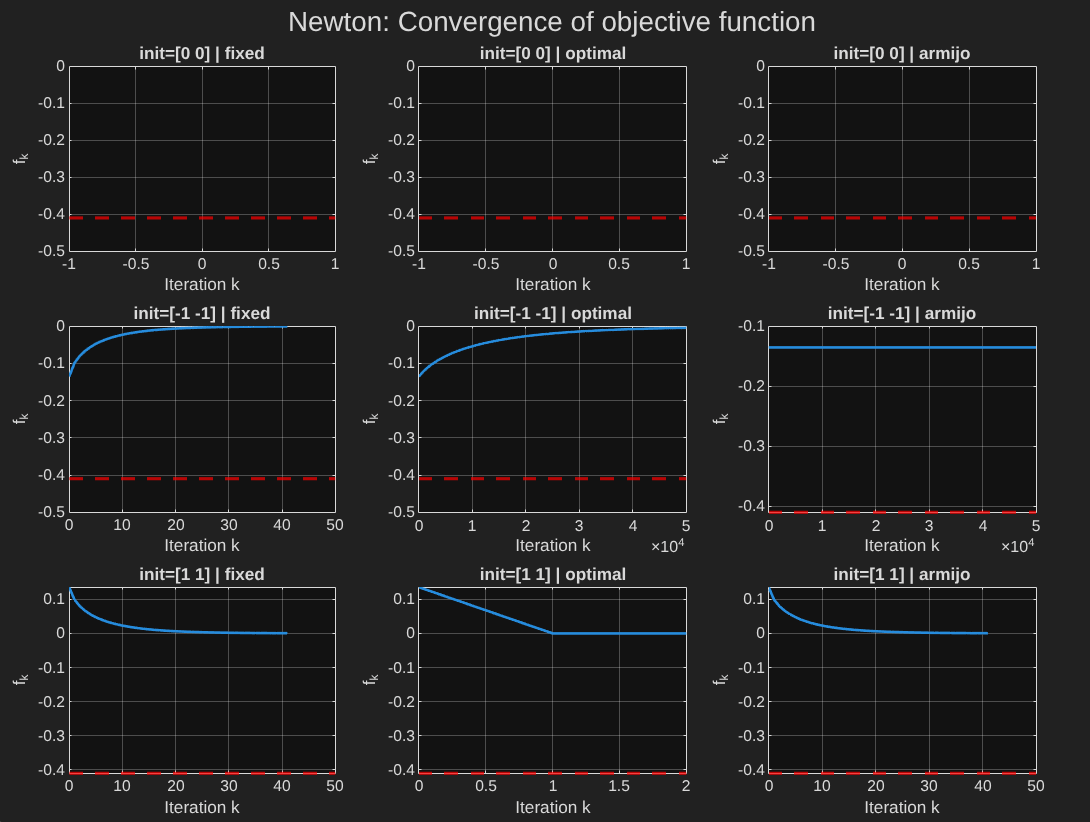
\includegraphics[width=0.95\textwidth]{assets/newton.png}
    \caption{Convergence of the objective function $f(x,y)$ for different step-size strategies.}
    \label{fig:newton}
\end{figure}

\subsection{Conclusions}

From the experiments with Newton's Method applied to the function $f$, several important observations can be made regarding the influence of the initial point and the choice of step-size strategy.

\paragraph{Initial point $(0,0)$}  
At this point, the Hessian matrix is singular, so its inverse cannot be computed. As a result, the method fails and returns NaN for all step-size strategies.

\paragraph{Initial point $(-1,-1)$}  
For this starting point, the behavior depends strongly on the step-size strategy:
\begin{itemize}
    \item \textbf{Fixed step:} Although the method converges quickly in 41 iterations, it moves the iterates far from the absolute minimum, reaching $(-0.615394, -1.544528)$ with $f \approx -0.000539$.
    \item \textbf{Optimal step:} The method converges to $(-0.712531, -1.406988)$ with $f \approx -0.004325$, but it requires the maximum number of iterations defined to terminate.
    \item \textbf{Armijo step:} The algorithm remains stuck at the initial point $(-1,-1)$ because the non-positive definite Hessian generates descent directions that are rejected by the Armijo condition.
\end{itemize}

\paragraph{Initial point $(1,1)$}  
The behavior is similar to Steepest Descent.  
\begin{itemize}
    \item The fixed step and Armijo strategies converge to $(0.615394, 1.544528)$ with $f \approx 0.000539$ in 41 iterations.  
    \item The optimal step converges to $(0.237173, 2.291851)$ with $f = 0$ in just 2 iterations.  
\end{itemize}  
None of these points correspond to the absolute minimum.

\paragraph{General Observations}  
\begin{itemize}
    \item Newton's Method is not effective for functions with a non-positive definite Hessian, such as the function in this study.  
    \item If the Hessian is singular, the method can produce NaN values and behave unpredictably.  
    \item The combination of the Armijo rule with Newton's Method can cause the algorithm to get stuck, as descent directions are sometimes rejected.  
    \item Overall, Newton's Method is highly sensitive to the choice of initial point and the definiteness of the Hessian matrix.
\end{itemize}

\section{Levenberg--Marquardt Method}

\subsection{Method Description}

The Levenberg--Marquardt method is designed to overcome one of the major weaknesses of Newton's Method: its reliance on a positive definite Hessian matrix.  
When the Hessian is not positive definite or is singular, Newton’s direction cannot be computed, and the method may diverge.  

To address this, the Levenberg--Marquardt method modifies the Hessian by adding a scaled identity matrix, resulting in the direction

\[
d_k = -\left[\nabla^2 f(x_k) + \mu_k I\right]^{-1} \nabla f(x_k),
\]

where $\mu_k > 0$ is a damping parameter.

Thus, the update rule becomes

\[
x_{k+1} = x_k - \gamma_k \left[\nabla^2 f(x_k) + \mu_k I\right]^{-1} \nabla f(x_k),
\]

where $\gamma_k$ is the step size determined by a fixed value, optimal line search, or Armijo rule.

The Levenberg--Marquardt method can be seen as a hybrid between Steepest Descent and Newton’s Method:
\begin{itemize}
    \item When $\mu_k$ is large, the term $\mu_k I$ dominates the Hessian.  
    In this case,
    \[
    \nabla^2 f(x_k) + \mu_k I \approx \mu_k I,
    \]
    and the update direction becomes similar to Steepest Descent.
    \item When $\mu_k$ is small, the Hessian term dominates and the method behaves like Newton’s Method.
\end{itemize}

In practice, $\mu_k$ is adapted dynamically. If the modified Hessian is not positive definite, $\mu_k$ is increased until positive definiteness is achieved. This ensures that the direction is always well-defined and descent-oriented.

\begin{algorithm}[H]
\caption{Levenberg--Marquardt Method}
\begin{algorithmic}[1]
\Require Function $f$, gradient $\nabla f$, Hessian $\nabla^2 f$, initial point $x_0$, damping parameter $\mu_0 > 0$, tolerance $\epsilon > 0$
\Ensure Approximate minimizer $x^*$
\State Set $x_k \gets x_0$, $\mu_k \gets \mu_0$, $k \gets 0$
\While{$\|\nabla f(x_k)\| > \epsilon$}
    \State Compute gradient $g_k = \nabla f(x_k)$
    \State Compute Hessian $H_k = \nabla^2 f(x_k)$
    \State Modify Hessian: $H^{LM}_k = H_k + \mu_k I$
    \State Ensure $H^{LM}_k$ is positive definite (increase $\mu_k$ if needed)
    \State Compute direction $d_k = - (H^{LM}_k)^{-1} g_k$
    \State Compute step size $\gamma_k$ (fixed, optimal, or Armijo)
    \State Update: $x_{k+1} \gets x_k + \gamma_k d_k$
    \State $k \gets k + 1$
\EndWhile
\State \Return $x^* \gets x_k$
\end{algorithmic}
\end{algorithm}

\subsection{Results}

In Table~\ref{table:lm} we present the numerical results obtained by 
applying the Levenberg--Marquardt method using the three step–size strategies: fixed step,
optimal step, and Armijo rule. 
For all experiments we used a termination threshold 
$\epsilon = 0.01$; for the fixed step strategy we set $\gamma = 0.1$, for the Armijo
rule we used the parameters $\alpha = 0.01$ and $\beta = 0.3$, and for damping parameter $\mu_0 = 0.1$.

\begin{table}[h!]
\centering
\begin{tabular}{c|c|c|c|c}
\textbf{Initial Point} & \textbf{Step Type} & \textbf{Minimum Point $x^*$} & \textbf{Minimum Value $f(x^*)$} & \textbf{Iterations} \\
\hline
$(0,0)$ & Fixed   & $(0,\;0)$      & $0$      & $1$ \\
$(0,0)$ & Optimal & $(0,\;0)$      & $0$      & $1$ \\
$(0,0)$ & Armijo  & $(0,\;0)$      & $0$      & $1$ \\
\hline
$(-1,-1)$ & Fixed   & $(-1.224719,\;-0.181756)$   & $-0.409469$     & $143$ \\
$(-1,-1)$ & Optimal & $(-1.224792,\;-0.165775)$   & $-0.409607$     & $5$ \\
$(-1,-1)$ & Armijo  & $(-1.224715,\;-0.182481)$   & $-0.409462$     & $570$ \\
\hline
$(1,1)$ & Fixed   & $(0.987044,\;1.589903)$      & $0.000609$      & $140$ \\
$(1,1)$ & Optimal & $(1.184497,\;1.706755)$      & $0.000084$      & $2$ \\
$(1,1)$ & Armijo  & $(0.982874,\;1.588684)$      & $0.000619$      & $553$ \\
\end{tabular}
\caption{Results of the Levenberg--Marquardt Method for different step-size strategies.}
\label{table:lm}
\end{table}

Figure~\ref{fig:lm} illustrates the convergence behavior of the 
objective function for all initial points and all step-size selection rules.

\begin{figure}[h!]
    \centering
    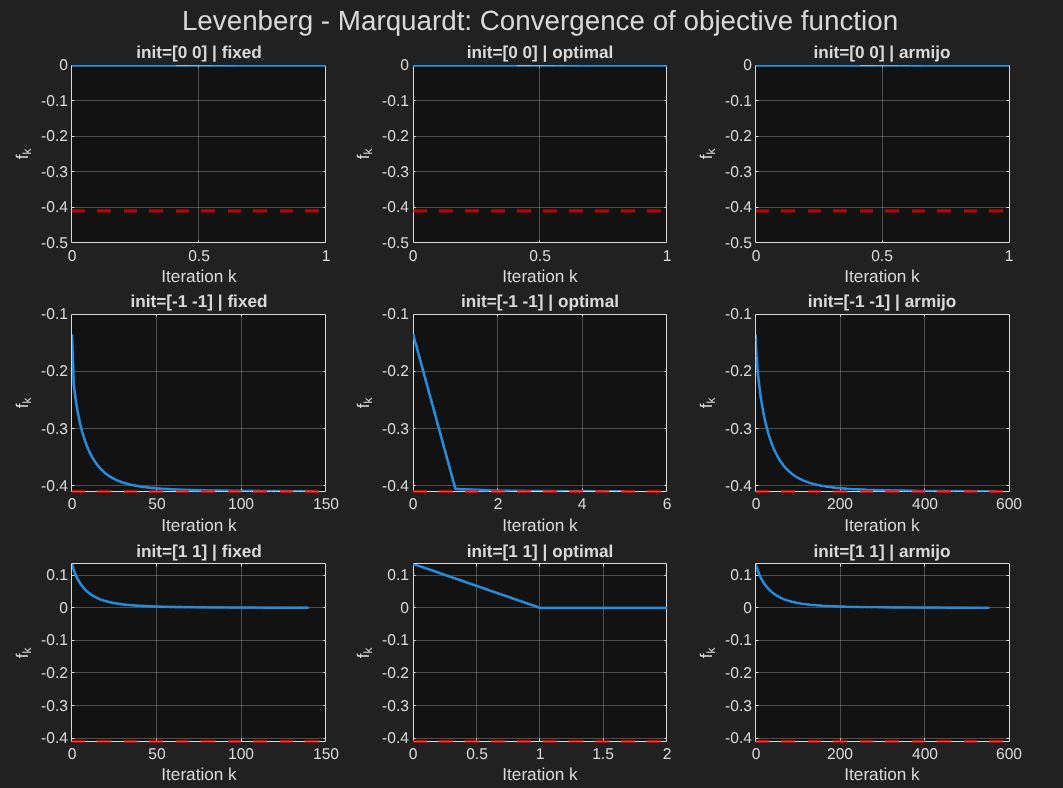
\includegraphics[width=0.95\textwidth]{assets/levenberg_marquardt.png}
    \caption{Convergence of the objective function $f(x,y)$ for different step-size strategies.}
    \label{fig:lm}
\end{figure}

\subsection{Conclusions}

From the experiments with the Levenberg--Marquardt method, we observe that the behavior of the algorithm is strongly influenced by the choice of initial point and by the damping mechanism that modifies the Hessian.

\paragraph{Initial point $(0,0)$}  
As in the previous methods, the point $(0,0)$ lies in a region where the gradient of the function is exactly zero.  
Therefore, the termination condition $\|\nabla f(x_k)\| < \epsilon$ is satisfied immediately, and the algorithm stops after the first iteration without progressing toward the actual minimizer.

\paragraph{Initial point $(-1,-1)$}  
For this initial point, the method successfully converges to the global minimum
\[
(x^*,y^*) \approx (-1.224570,\,-0.0887658), 
\qquad 
f(x^*,y^*) = -0.4098908.
\]
However, the number of iterations required varies significantly across the three step-size strategies:  
143 iterations for the fixed step, 5 iterations for the optimal step, and 570 iterations for the Armijo rule.

Compared to Steepest Descent, the Levenberg--Marquardt method requires substantially more iterations for the fixed and Armijo strategies.  
This behavior is expected: LM modifies the Hessian at every iteration by adding $\mu_k I$, and when $\mu_k$ becomes relatively large (in order to enforce positive definiteness), the update direction becomes closer to
\[
d_k \approx -\frac{1}{\mu_k}\,\nabla f(x_k),
\]
which resembles a \emph{scaled} Steepest Descent direction with a very small effective step size.  
Thus, when the Hessian is poorly conditioned or far from positive definite—as happens in large regions of this function—the LM method tends to move cautiously, often requiring many iterations before reaching the valley of the minimum.

On the other hand, when $\mu_k$ becomes small, the method approaches Newton's behavior and converges significantly faster.

\paragraph{Initial point $(1,1)$}  
As with the previous methods, starting from the point $(1,1)$ does not lead to the global minimum.  
The fixed and Armijo steps converge to the local region around  
\[
(0.982874,\;1.588684), \qquad f \approx 0.000619,
\]
in 140 and 553 iterations respectively, while the optimal step reaches the point  
\[
(1.184497,\;1.706755), \qquad f \approx 0.000084,
\]
in only 2 iterations.  
All these values correspond to flat, nearly constant regions near the “hill” of the function and not to its global valley on the left side.

\paragraph{General Observations}
\begin{itemize}
    \item The LM method is more robust than Newton’s Method because it ensures that the modified Hessian is always invertible and positive definite.
    
    \item However, robustness comes at the cost of speed: when the damping parameter $\mu_k$ becomes large, the update direction resembles a very cautious Steepest Descent step, which dramatically slows convergence.

    \item The method performs best when the optimal step strategy is used.

    \item When the starting point is far from the global minimum (e.g., $(1,1)$), the method may converge to flat regions where the gradient is nearly zero.

    \item Overall, Levenberg--Marquardt is effective and reliable near the global minimum, but its hybrid nature may lead to significantly more iterations than Steepest Descent in regions where the Hessian is indefinite or poorly conditioned.
\end{itemize}

\section{Overall Comparison of the Methods}

To conclude this study, we summarize the behavior of the three optimization methods—Steepest Descent, Newton’s Method, and Levenberg--Marquardt—across the three initial points and step–size strategies. The table below provides a compact overview, followed by general observations regarding convergence speed, robustness, and sensitivity to initialization.

\subsection*{Summary Table}

\begin{table}[H]
\centering
\begin{tabular}{c|c|c|c|c}
\textbf{Method} & \textbf{Init. Point} & \textbf{Step Type} & \textbf{Found Minimum?} & \textbf{Iterations} \\
\hline
\multirow{9}{*}{Steepest Descent}
& $(0,0)$ & All & No (stops immediately) & 1 \\
& \multirow{3}{*}{$(-1,-1)$}
& Fixed   & Yes & 92 \\
& & Optimal & Yes & 2 \\
& & Armijo  & Yes & 92 \\
& \multirow{3}{*}{$(1,1)$}
& Fixed   & No & 89 \\
& & Optimal & No & 2 \\
& & Armijo  & No & 89 \\
\hline
\multirow{9}{*}{Newton}
& $(0,0)$ & All & No (Hessian singular) & 1 \\
& \multirow{3}{*}{$(-1,-1)$}
& Fixed   & No & 41 \\
& & Optimal & No & 50000 \\
& & Armijo  & No & 50000 \\
& \multirow{3}{*}{$(1,1)$}
& Fixed   & No & 41 \\
& & Optimal & No & 2 \\
& & Armijo  & No & 41 \\
\hline
\multirow{9}{*}{Levenberg--Marquardt}
& $(0,0)$ & All & No (stops immediately) & 1 \\
& \multirow{3}{*}{$(-1,-1)$}
& Fixed   & Yes & 143 \\
& & Optimal & Yes & 5 \\
& & Armijo  & Yes & 570 \\
& \multirow{3}{*}{$(1,1)$}
& Fixed   & No & 140 \\
& & Optimal & No & 2 \\
& & Armijo  & No & 553 \\
\end{tabular}
\caption{Summary comparison of the three optimization methods across all experiments.}
\end{table}

\subsection{General Conclusions}

\paragraph{Steepest Descent}
\begin{itemize}
\item Most reliable in reaching the global minimum when starting near the valley of the function.
\item Very slow convergence for fixed and Armijo step sizes; dramatically faster with optimal step.
\item Sensitive to regions where the gradient becomes small (e.g., near $(1,1)$), easily getting stuck in flat regions.
\end{itemize}

\paragraph{Newton’s Method}
\begin{itemize}
\item Highly efficient only when the Hessian is positive definite and the starting point is close to the minimizer (which does not hold for this function in most regions).
\item Fails completely at points where the Hessian is singular or indefinite.
\item Extremely sensitive to the initial point; may diverge or stagnate.
\item Fast convergence (2 iterations) only occurs in regions where the quadratic model is well-behaved—yet still converges to incorrect regions of the domain.
\end{itemize}

\paragraph{Levenberg--Marquardt}
\begin{itemize}
\item The most robust method: it never fails due to Hessian singularities because the modified Hessian is always invertible.
\item Successfully converges to the global minimum from $(-1,-1)$ under all step–size strategies.
\item When the damping parameter is large, the method behaves like a conservative Steepest Descent scheme, leading to many iterations (especially with Armijo).
\item When the damping parameter is small, the method resembles Newton's Method and converges much faster.
\item Still fails to escape flat regions when starting far from the valley of the global minimum.
\end{itemize}

\subsection{Overall Comparison}

\begin{itemize}
\item \textbf{Best method for robustness:}  
Levenberg--Marquardt, since it handles singular or indefinite Hessians and always produces a well-defined descent direction.

\item \textbf{Best method for speed:}  
Steepest Descent with optimal step size, which converges in just 2 iterations.

\item \textbf{Best method for reaching the global minimum:}  
Steepest Descent and Levenberg--Marquardt, but only when initialized near $(-1,-1)$.

\item \textbf{Worst overall performance:}  
Newton’s Method, due to extreme sensitivity to Hessian definiteness and failure at singular points.

\item \textbf{Most sensitive to initialization:}  
All three methods.  
Because the function contains flat regions and strong curvature variations, none of the methods successfully moves from $(1,1)$ to the global minimum.
\end{itemize}

\end{document}
